\section{Oferirea accesului unui utilizator}

Opera'tia de oferire a accesului unui nou utilizator presupune folosirea interfe'tei de administrare. După setarea numeului de utilizator 'si a parolei, noul cont este gata pentru folosit, iar pentru convenabilitate codul QR generat poate fi scanat cu aplica'tia pentru a se autentifica automat.

\begin{figure}[H]
\begin{center}
  \subfloat[Introducerea credentialelor noi]{\label{fig:useradda}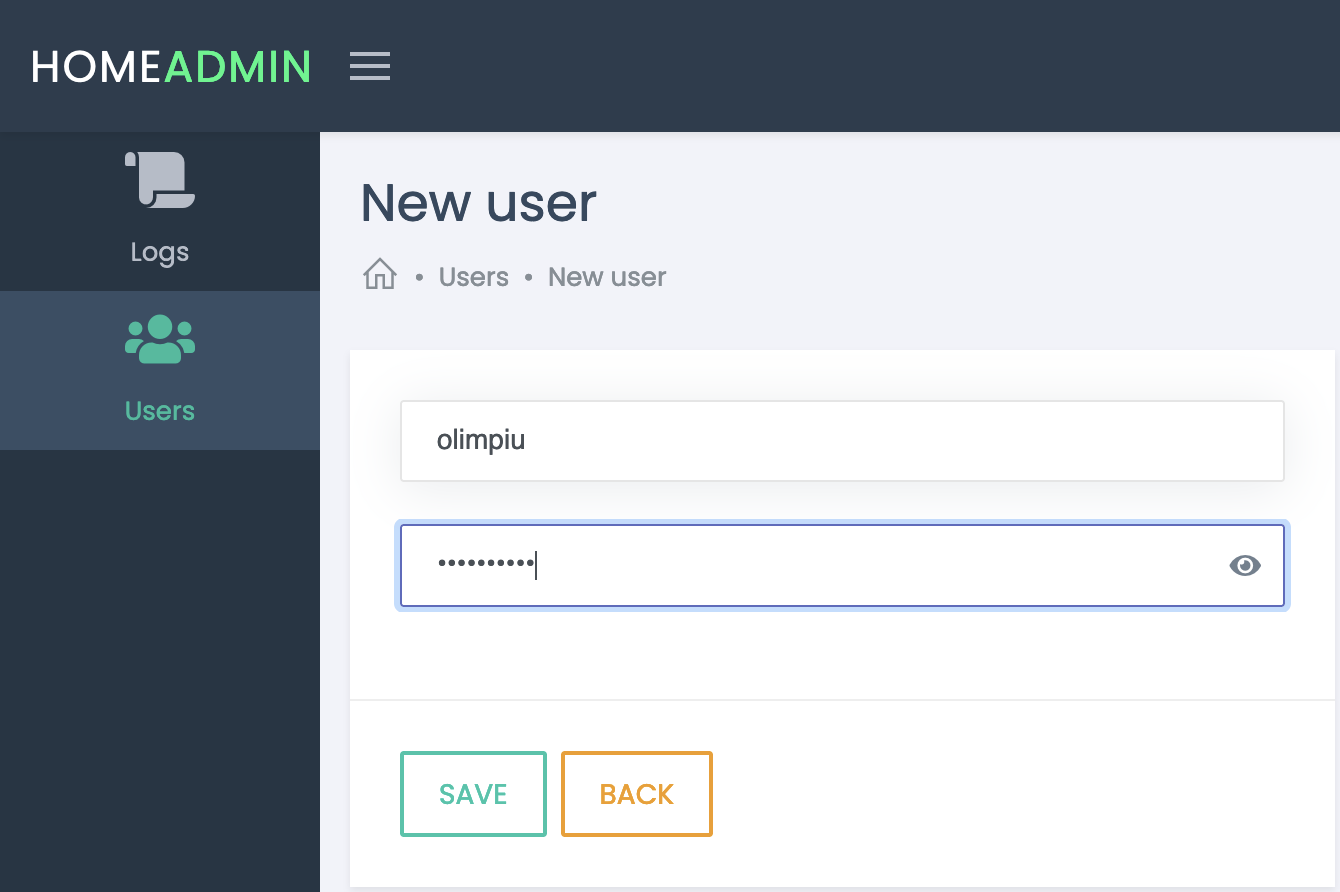
\includegraphics[width=\doublefigure]{05/06_admin_add_user.png}}
  \hfil
  \subfloat[Confirmarea adăugării noului cont]{\label{fig:useraddb}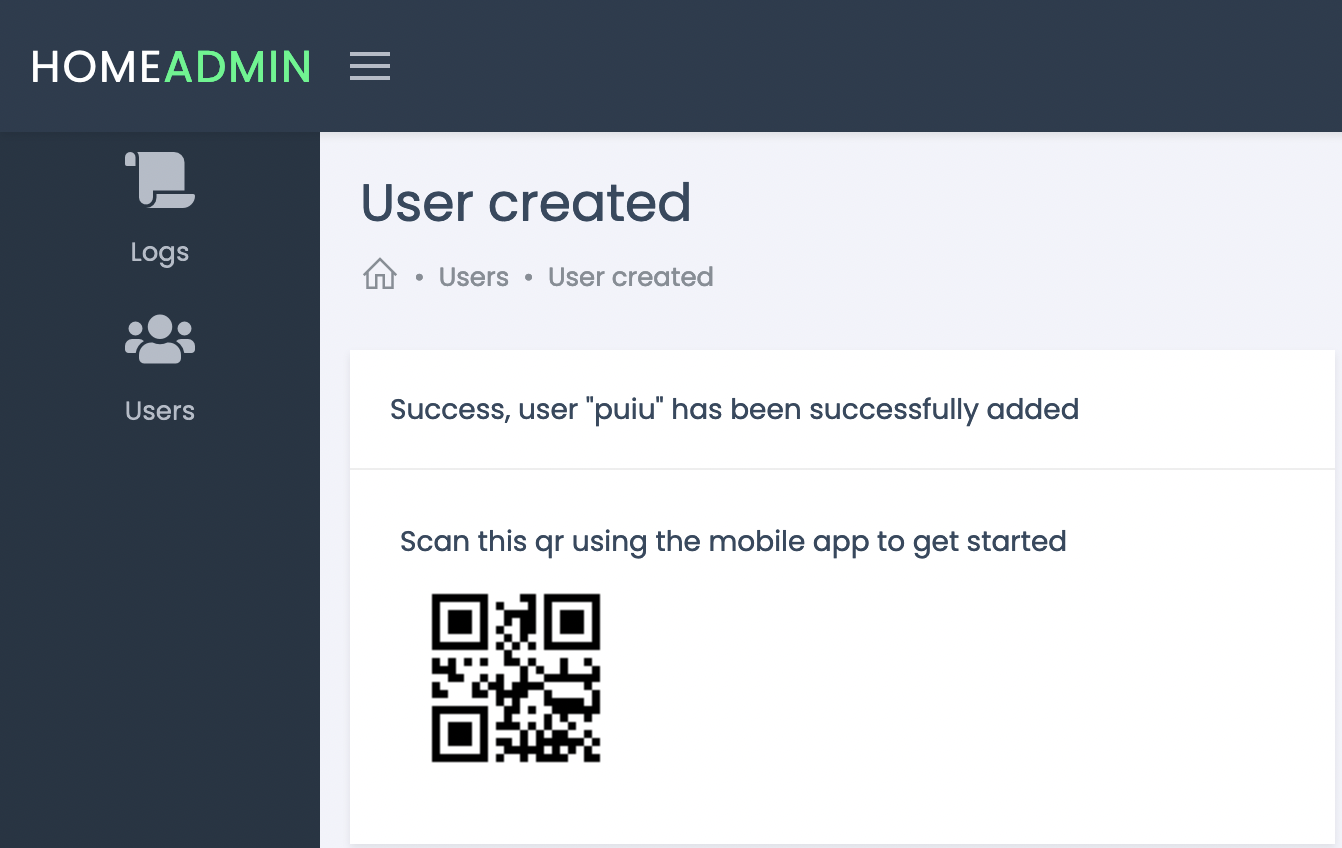
\includegraphics[width=\doublefigure]{05/07_admin_add_user_success.png}}
  \caption{Creare utilizator nou}
  \label{fig:useradd}
\end{center}
\end{figure}

După descărcarea aplica'tiei din Google Play Store, se va putea realiza autentificarea. Un alt avantaj al unui astfel de sistem este eliminarea nevoii cartelelor fizice, u'sor pierdut sau încurcat.

\begin{figure}[H]
\begin{center}
  \subfloat[Ecran autentificare aplica'tie]{\label{fig:androidqra}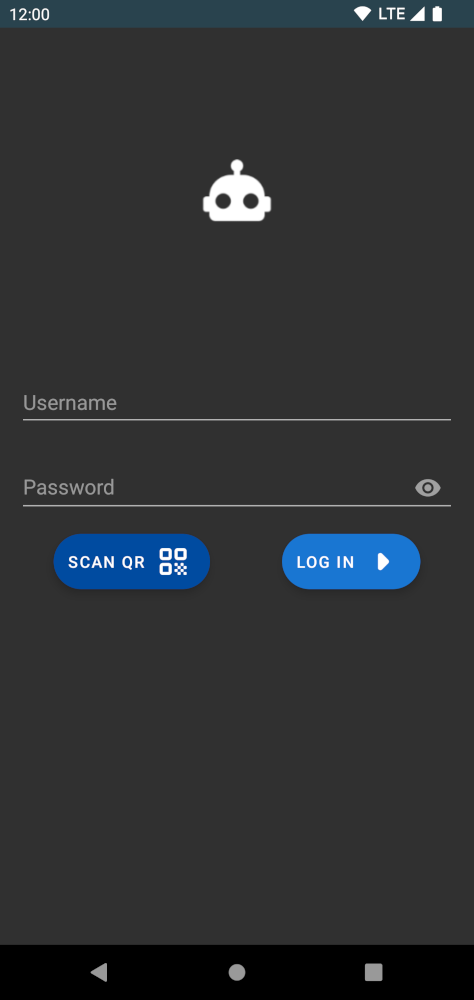
\includegraphics[width=\doublefigure]{05/08_android_log_in.png}}
  \hfil
  \subfloat[Scanarea codului QR]{\label{fig:androidqrb}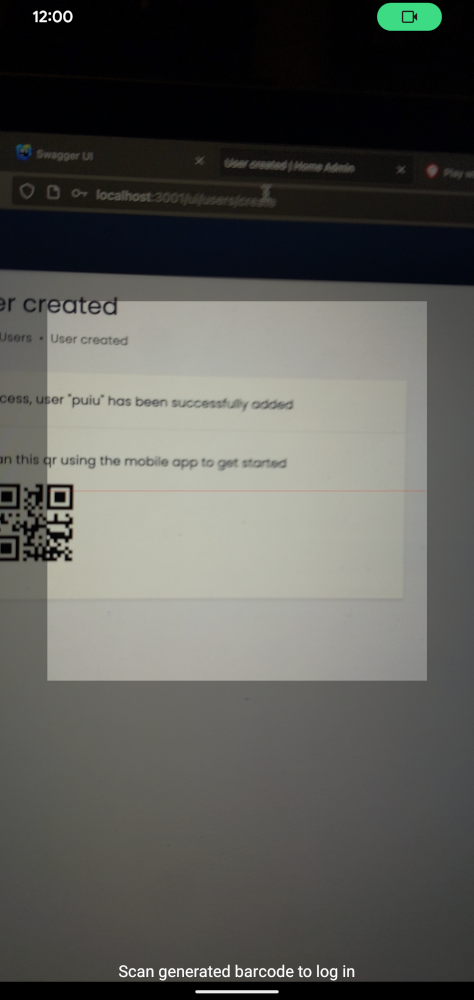
\includegraphics[width=\doublefigure]{05/09_android_qr.png}}
  \caption{Autentificare prin scanare cod QR}
  \label{fig:androidqr}
\end{center}
\end{figure}

\section{Răspuns automat}

Majoritatea vizitelor 'si apelurilor la interfon sunt predictibile, de exemplu venirea curierului sau a unui po'sta's este anun'tată printr-un interval aproximativ de timp. Deoarece utilizatorul duce o via'tă ocupată 'si 'stie că urmează să fie sunat, poate programa sistemul să răspundă 'si să deschidă automat u'sa la următorul apel pentru o durată predefinita.

\begin{figure}[H]
\begin{center}
  \subfloat[Apăsarea butonului albastru auto-answer va arăta meniul pentru configurarea func'tionalită'tii]{\label{fig:autoanswera}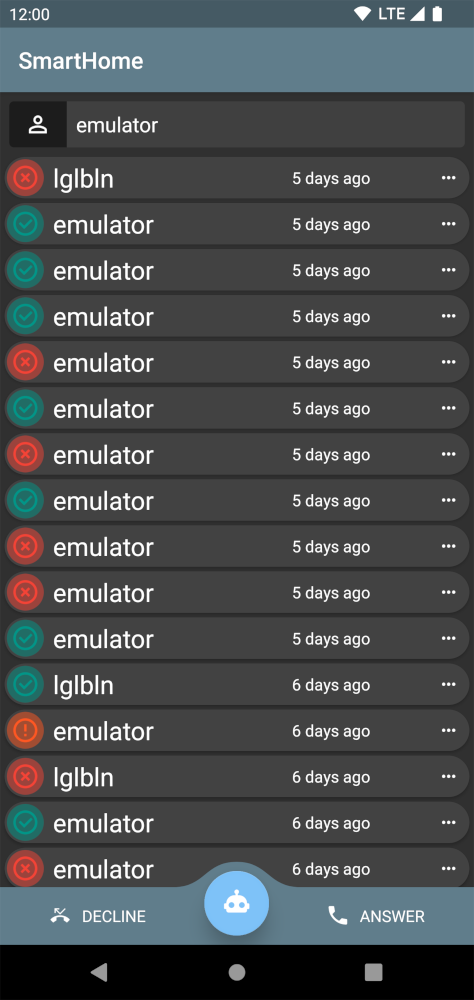
\includegraphics[width=\doublefigure]{05/01_android_autoanswer.png}}
  \hfil
  \subfloat[Alegerea unui interval pentru care func'tia va fi activă]{\label{fig:autoanswerb}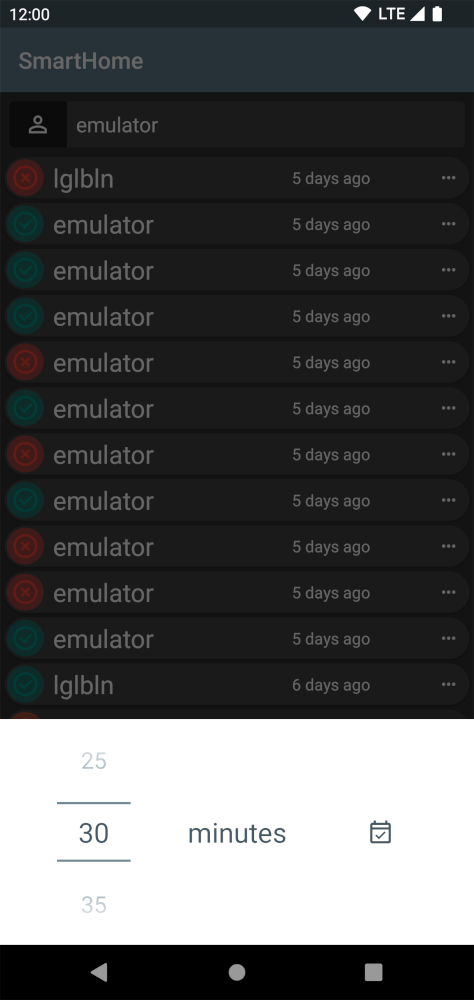
\includegraphics[width=\doublefigure]{05/02_android_auto_set.png}}
  \caption{Pa'si pentru setare func'tie auto-answer}
  \label{fig:autoanswer}
\end{center}
\end{figure}

Se confirmă activarea func'tiei prin colorarea butonului auto-answer în portocaliu. Într-o maniera similiara, daca se dore'ste oprirea înainte de termen, se poate face acest lucru din meniul anterior.

\section{Răspuns de la distanta}

Prin conectarea la re'teaua \acrshort{iot} sistemul este expus Internetului, acesta fiind avantajul solu'tiei, dar 'si unul din factorii limitanti ai sai. Posibilitatea de deschidere de oriunde clientul are un dispzitiv conectat la Internet înseamnă că în lipsa cartelei standard \acrfull{rfid} se poate apela propriul apartament. Se va folosi aplica'tia mobila pentru a se raspunde la propriul apel.

\begin{figure}[H]
\begin{center}
  \subfloat[În cazul în care aplica'tia este pornită, utilizatorul este redirectat în IncomingActivity]{\label{fig:ringinga}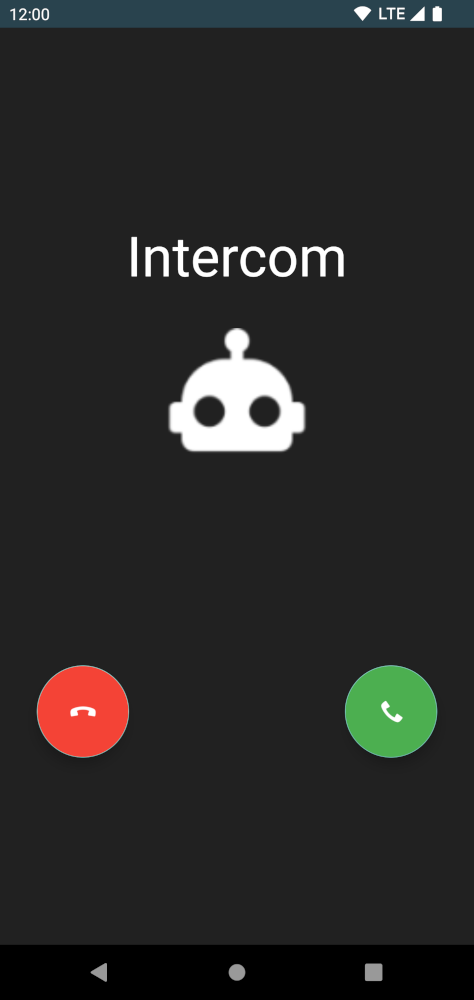
\includegraphics[width=\doublefigure]{05/04_android_app_ringing.png}}
  \hfil
  \subfloat[În cazul în care aplica'tia nu este în foreground, se trimite o notificare de sistem cu două ac'tiuni]{\label{fig:ringingb}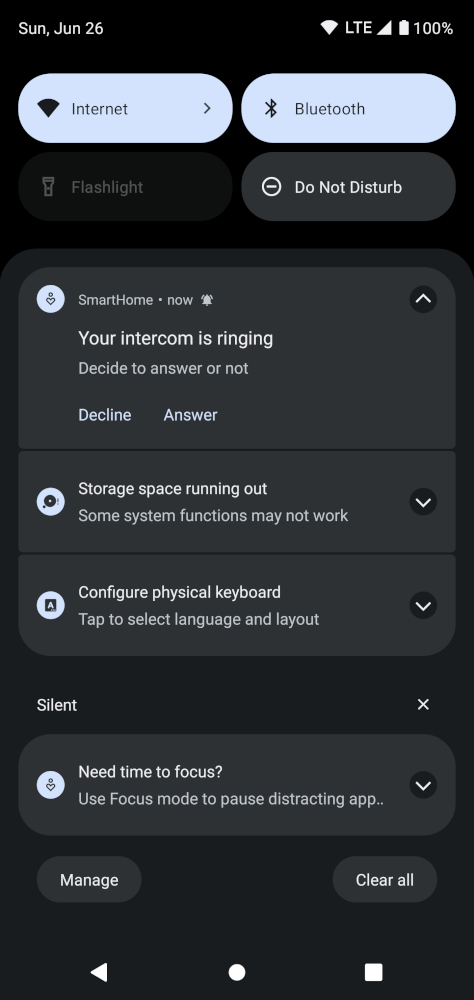
\includegraphics[width=\doublefigure]{05/05_android_notification_ringing.png}}
  \caption{Ecran apel}
  \label{fig:ringing}
\end{center}
\end{figure}

O altă variantă pentru mitigarea acestei probleme a fost folosirea unui tag \acrfull{nfc} care con'tine codat url-ul de acces împreună cu un token care nu expiră. Astfel prin scanarea lui cu un telefon ce dispune de antenă \acrshort{nfc} se va realiza request-ul din browserul default al utilizatorului, rezultând în deschiderea interfonului.